\documentclass[exercice]{thedocument}%
\begin{document}%
\>figure1={\begin{tikzpicture}[scale=1.5]%
    \coordinate[label=below left:F](A)at(0,0);
    \coordinate[label=right:J](B)at(20:2);
    \coordinate[label=E](C)at(60:2);
    \draw(A)--(B)--(C)--cycle;
    \tkzMarkSegment[mark=s||](A,B)
    \tkzMarkSegment[mark=s||](A,C)
\end{tikzpicture}};%
\>figure2={\begin{tikzpicture}[scale=1.5]%
    \coordinate[label=above:H](A)at(0,0);
    \coordinate[label=below left:J](B)at(-120:2);
    \coordinate[label=right:K](C)at(-30:2);
    \draw(A)--(B)--(C)--cycle;
    \tkzMarkSegment[mark=s||](A,B)
    \tkzMarkSegment[mark=s||](A,C)
    \tkzMarkRightAngle(B,A,C)
    \path(B)--(A)node[above,pos=0.5,sloped,yshift=10pt]{12 dm};
\end{tikzpicture}};%
\>figure3={\begin{tikzpicture}[scale=0.75]%
    \coordinate[label=below left:G](A)at(0,0);
    \coordinate[label=below right:K](B)at(4,0);
    \coordinate[label=above right:E](C)at(4,3);
    \coordinate[label=above left:A](D)at(0,3);
    \draw(A)--(B)--(C)--(D)--cycle;
    \tkzMarkSegment[mark=s||](A,B)
    \tkzMarkSegment[mark=s||](C,B)
    \tkzMarkSegment[mark=s||](C,D)
    \tkzMarkSegment[mark=s||](A,D)
    \path(D)--(C)node[above,pos=0.5,sloped,yshift=10pt]{2,1 cm};
\end{tikzpicture}};%
\>figure4={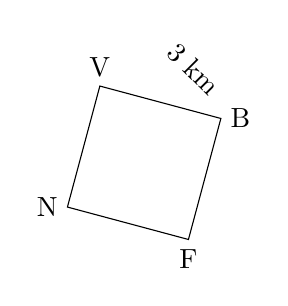
\begin{tikzpicture}[scale=0.75,rotate=30]%
    \coordinate[label=right:B](A)at(0:1.5);
    \coordinate[label=above:V](B)at(90:1.5);
    \coordinate[label=left:N](C)at(180:1.5);
    \coordinate[label=below:F](D)at(-90:1.5);
    \draw(A)--(B)--(C)--(D)--cycle;
    \tkzMarkSegment[mark=s||](A,B)
    \tkzMarkSegment[mark=s||](C,B)
    \tkzMarkSegment[mark=s||](C,D)
    \tkzMarkSegment[mark=s||](A,D)
    \tkzMarkRightAngle(A,B,C)
    \tkzMarkRightAngle(B,C,D)
    \tkzMarkRightAngle(C,D,A)
    \tkzMarkRightAngle(D,A,B)
    \path(A)--(B)node[above,pos=0.5,sloped,yshift=10pt]{3 km};
\end{tikzpicture}};%
\enonce{0499}%
\end{document}